% !TeX root = ../../../main.tex
\begin{figure}[htbp]
\begin{ChEightFloatBody}

    \centering
    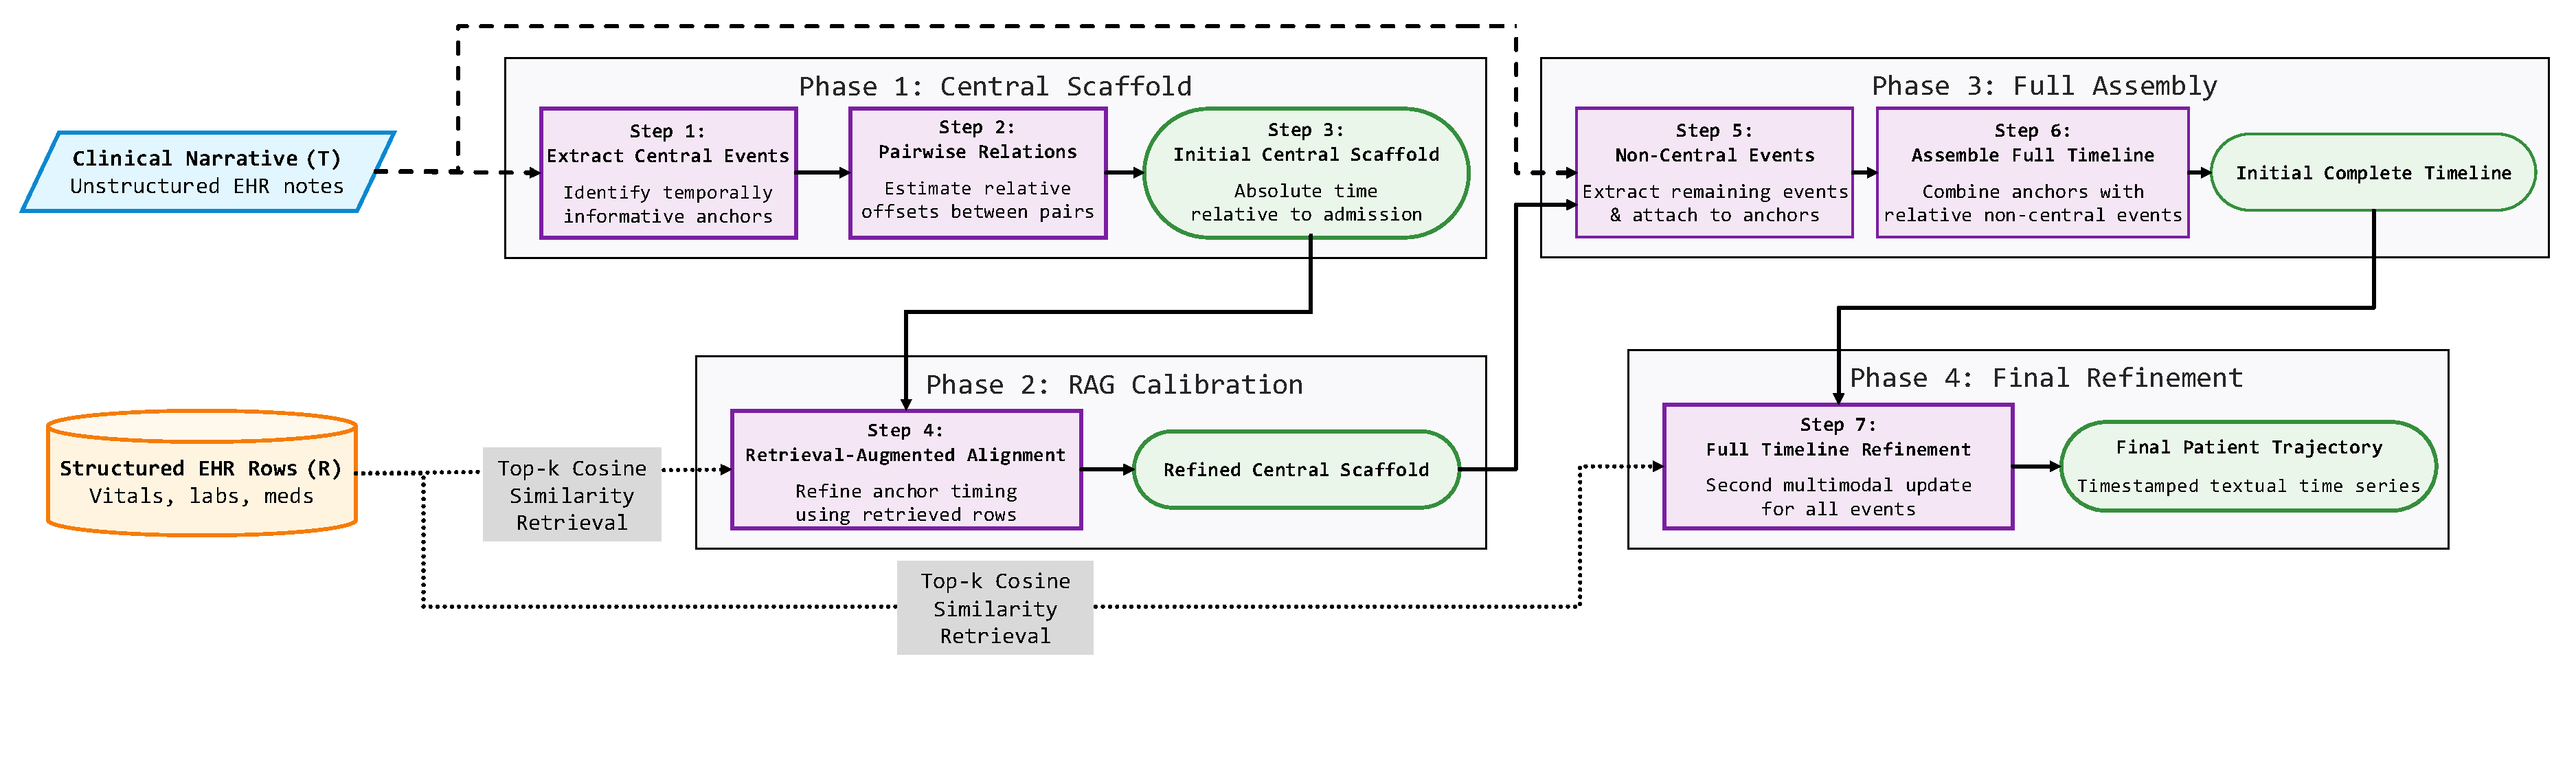
\includegraphics[width=\textwidth]{Chapters/chapter-08/images/plots/TTA-Overview-Figure-Model-Updated.pdf}
    
    
    
    

\end{ChEightFloatBody}
\caption{
    Overview of the scaffolded retrieval-augmented timeline reconstruction workflow. The method first extracts central events from the clinical narrative, estimates pairwise temporal relations, and builds an initial central-event scaffold. Retrieved structured EHR rows are then used to calibrate this scaffold. Non-central events are extracted and attached relative to central events, after which a final retrieval-augmented refinement step calibrates the complete timeline.
    % \textcolor{blue}{Shahriar-update figure to remove symbols if relevant}
    }\ChEightFloatLabel{ch08:fig:pipeline}
\end{figure}